\documentclass{standalone}
  \usepackage{tikz}
  \usetikzlibrary{arrows.meta, automata, bending, positioning, shapes.misc}
  \tikzstyle{automaton}=[shorten >=1pt, >={Stealth[bend,round]}, initial text=]
  \tikzstyle{accepting}=[accepting by arrow]

\begin{document}
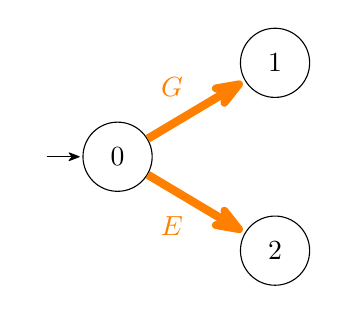
\begin{tikzpicture}[automaton, auto]
  \node[state,initial,rounded rectangle] (0) {$0$};
  \node[state,rounded rectangle] (1) [above right=3mm and 20mm of 0] {$1$};
  \node[state,rounded rectangle] (2) [below right=3mm and 20mm of 0] {$2$};
  \path[->] (0) edge[orange,line width=3] node {$G$} (1);
  \path[->] (0) edge[orange,line width=3] node[swap] {$E$} (2);
\end{tikzpicture}
\end{document}
